\section{Sistemi lineari}
Un \textbf{sistema} fisico è un apparato che riceve in input un segnale e ne produce un altro in output. Questa interazione è descritta da una funzione (operatore), le cui caratteristiche determinano il segnale in uscita. Il processo contiene una relazione di ingresso-uscita, o causa-effetto.
$$y(t) = S[x(t)]$$
Il campionamento con periodo o frequenza è un esempio di sistema, applicando un campionatore che legge istanti continui e li trasforma in discreti in base al passo $\Delta t$. 

Un altro esempio è il quantizzatore, che associa al segnale $f(t)$ il segnale $Q(t)$ dove $Q$ indica l'elemento in $V = \{x_1, \dots, x_n\}$ più vicino al numero reale $x$ (valori finiti).

I sistemi possono avere più ingressi e uscite, come la somma $g(t) = f(t) + h(t)$. Mettendo insieme più sistemi semplici, ne vengono generati di più complessi in diversi combinazioni di componenti elementari:
\begin{itemize}
	\item \textbf{Composizione sequenziale} (a cascata), che combina più sistemi di cui l'output di uno è l'input di un altro (come processo di digitalizzazione);
	\item \textbf{Composizione parallela}, in cui lo stesso input viene immesso in più sistemi diversi;
	\item \textbf{Retroazione}, in cui l'output di un sistema viene modificato da un'altra funzione e torna come input della precedente (il risultato dipende dai valori precedenti).
\end{itemize}

Un sistema a tempo discreto è un dispositivo che trasforma una sequenza $x(n)$ in ingresso in una sequenza di uscita $y(n)$, attraverso un operatore $L[\cdot]$ (relazione di I/O). L'operatore è descrivibile tramite una sequenza, che definisce le proprietà del sistema.

\subsection{Composizioni}
\subsubsection{Cascata}
Dati due sistemi $S1 : F1 \rightarrow F2$ e $S2 : F2 \rightarrow F3$, la loro composizione sequenziale è il sistema $S3 : F1 \rightarrow F3$ ottenuto ponendo in ingresso a $S2$ la risposta di $S1$.

\begin{figure}[h]
	\centering
	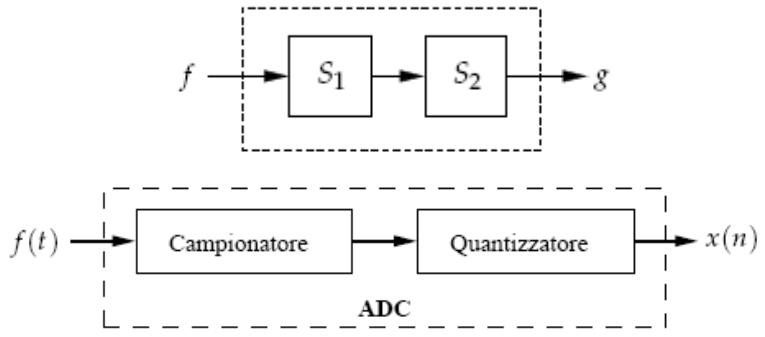
\includegraphics[scale=0.4]{Lezioni/Immagini/cascata}
\end{figure}

\subsubsection{Parallela}
Dati due sistemi $S1 : F1 \rightarrow F2$ e $S2 : F2 \rightarrow F3$, la loro composizione parallela è il sistema che ha come risposta la somma delle risposte di $S1$ e $S2$.

Perché si possa definire la composizione parallela, deve succedere che la somma di due segnali in $F2$ sia ancora un segnale in $F2$.

\begin{figure}[h]
	\centering
	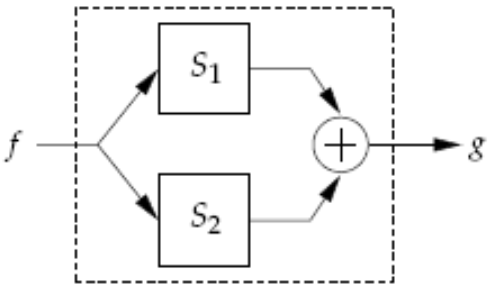
\includegraphics[scale=0.4]{Lezioni/Immagini/parallela}
\end{figure}

\subsubsection{Retroazione}
Dati due sistemi $S1 : F1 \rightarrow F2$ e $S2 : F2 \rightarrow F3$, il sistema ottenuto per retroazione è il sistema $S3$ che ha ingresso $f$ e uscita $g$ ottenuta ponendo in ingresso a $S1$ la differenza tra $f$ e la risposta di $S2$ a $g$.

\begin{figure}[h]
	\centering
	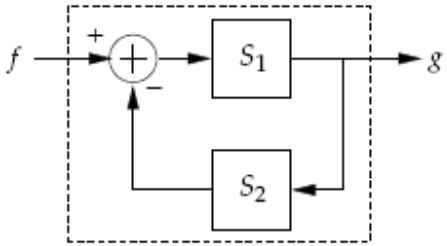
\includegraphics[scale=0.4]{Lezioni/Immagini/retroazione}
\end{figure}

\subsection{Tempo-invarianza}
Un sistema complesso lineare può sempre essere scomposto in \textit{componenti semplici}, e questo principio può essere applicato anche sugli input (più sistemi) con lo stesso operatore sui segnali. La relazione I/O soddisfa il principio di \textbf{sovrapposizione degli effetti}. 

Dato il segnale in ingresso $x(n) = \alpha_1x_1(n) + \alpha_2x_2(n)$, la risposta a una combinazione lineare di ingressi è la combinazione lineare delle risposte del sistema ai singoli ingressi.
$$L[x(n)] = L[\alpha_1x_1(n) + \alpha_2x_2(n)] = \alpha_1L[x_1(n)] + \alpha_2L[x_2(n)]$$
Un'altra proprietà dei sistemi è la \textbf{tempo-invarianza}: sono stazionari e rispondono nello stesso modo in istanti differenti, quindi l'output è lo stesso anche con ritardo. 

La relazione I/O produce un segnale di uscita $y(n)$ che dipende solo dalla forma del segnale di ingresso $x(n)$:
$$L[x(n - n_0)] = y(n - n_0)$$
Se l'ingresso al sistema è ritardato o anticipato di una quantità $n_0$, allora anche la risposta viene ritardata o anticipata di $n_0$.

Sistemi \textbf{causali}: presupponendo il campione attuale e i successivi, la risposta corrente $x(n)$ non dipende dai valori futuri $x(n + n_0)$ con costante intera $n_0 > 0$ (solo parte positiva).

Sistemi \textbf{anticausali}: considerando il campione corrente e i precedenti, la risposta corrente $y(n)$ non dipende dai valori passati $x(n - n_0)$ con costante intera $n_0 > 0$ (solo parte positiva). Non  sono fisicamente realizzabili.

I sistemi \textbf{bilateri} hanno sia parte causale che anticausale.

I sistemi possono avere \textbf{memoria}, la cui grandezza è il numero di campioni che vengono immagazzinati per calcolare i risultati successivi. La risposta corrente in questo caso dipende dai valori dell'ingresso negli istanti di tempo precedenti a quello corrente $n$ (altrimenti sono statici).

Un sistema a tempo discreto si dice \textit{passivo} quando l'energia $E_y$ dell'output $y(n)$ è minore o uguale all'energia $E_x$ dell'input $x(n)$. Questo si rappresenta con il modulo quadro, osservando la conservazione. 
$$\sum_{n=-\infty}^{+\infty}\abs{y(n)}^2 \leq \sum_{n=-\infty}^{+\infty}\abs{x(n)}^2 < \infty$$
Se la relazione precedente vale con il segno di uguaglianza, allora il sistema è detto \textit{senza perdite}, in quanto conserva l'energia del segnale di ingresso.

\subsection{Sistemi LTI}
I \textbf{sistemi lineari tempo invariante} (LTI) sono definiti da operazioni I/O che soddisfano contemporaneamente la \textbf{linearità} e la \textbf{stazionarietà}. Se i coefficienti sono costanti, il segnale è stazionario perché non cambia in funzione al peso.

L'analisi dei LTI può essere condotta in tre diversi modi:
\begin{enumerate}
	\item \textit{Relazione I/O} (qualsiasi sistema);
	\item \textit{Equazione lineare alle differenze a coefficienti costanti }(LTI causale);
	\item \textit{Risposta all'impuls}o nel dominio del tempo e delle frequenze (sistema LP).
\end{enumerate}

In particolare per il caso di equazione alle differenze, l'output è espresso come combinazione lineare di tutti i valori (coefficienti reali, costanti positive o negative) della sequenza di input $x(n)$, che è combinazione lineare della stessa sequenza di output, a partire dal primo campione ritardato. 
$$y(n) = -\alpha_1y(n-1) - \alpha_2y(n - 2) - \ldots - \alpha_My(n - M) + \beta_0x(n) + \beta_1x(n - 1) + \ldots + \beta_Nx(n - N)$$
L'uscita $y(n)$ dipende sia dai valori che l'ingresso $x(n)$ assume in un arco temporale fino a $N$ istanti precedenti all'istante di tempo discreto $n$, sia dai valori assunti dal segnale di uscita $y(n)$ fino a $M$ istanti di tempo precedenti a quello corrente $n$.

Queste operazioni possono essere raccolte come sommatoria con coefficienti costanti indipendenti dal tempo:
$$y(n) = \sum_{k=0}^{N} \beta_kx(n - k) - \sum_{j=1}^{M} \alpha_jy(n - j)$$
La $y$ non parte da zero perchè altrimenti $y(n)$ dovrebbe dipendere da se stessa. Se l'equazione è ricorsiva (almeno un coefficiente $\alpha_j$ diverso da zero), la memoria è infinita.

Un'altra modalità per descrivere un sistema lineare a tempo invariante è la risposta all'impulso: la relazione I/O è semplice perché si indica la reazione alla $\delta$, dove il peso è il valore della sequenza in quel campione. Essendo lineare a tempo invariante, i segnali sono indipendenti dal tempo e esprimibili come combinazioni lineari. 

L'analisi della risposta del sistema all'impulso permette di valutare la risposta a regime, al fine di semplificarne l'analisi tempo-frequenza rappresentando la sequenza come somma di $\delta$ traslate e pesate.
$$x(n) = \sum_{i=-\infty}^{+\infty}x(i)\delta(n-i)$$
Per la proprietà di sovrapposizione degli effetti (linearità) e di stazionarietà, si ha:
$$y(n) = L\Big[\sum_{i=-\infty}^{\infty}x(i)\delta(n - i)\Big] = \sum_{i=-\infty}^{\infty}x(i)L[\delta(n - i)] = \sum_{i=-\infty}^{\infty}x(i)h(n - i) = x * h$$
$h$ è il kernel, la sequenza che descrive il comportamento del filtro (risposta del sistema all'impulso). La formula si può ritrovare come \textbf{convoluzione} lineare discreta della sequenza con il filtro.

\begin{figure}[h]
	\centering
	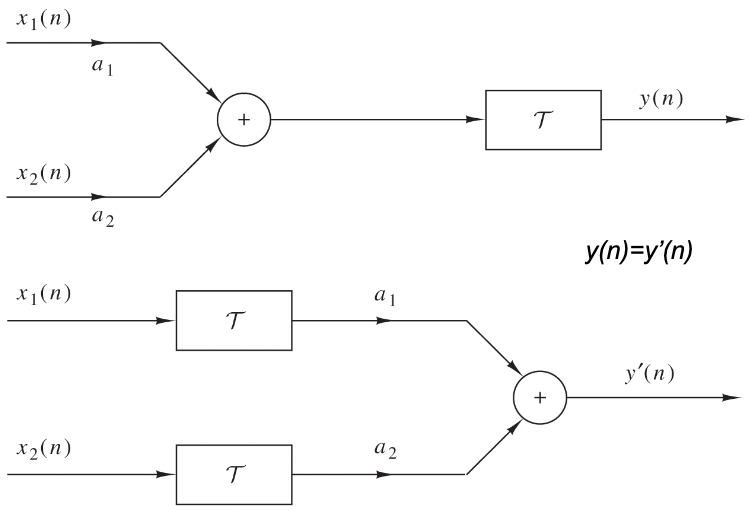
\includegraphics[scale=0.35]{Lezioni/Immagini/sovrapposizione}
\end{figure}

Se i segnali sono causali e limitati, il numero di valori sarà finito. La risposta all'impulso $h(n)$ è nulla per istanti di tempi $n < 0$, e l'uscita dipende dal valore corrente del segnale d'ingresso $x(n)$ e dei campioni già presenti nel sistema. 

Se la risposta all'impulso $h(n)$ ha supporto temporale finito $N_h$, l'uscita del sistema LTI è:
$$y(n) = x(n) * h(n) = \sum_{i=0}^{N_h-1}h(i)x(n - i)$$
L'operatore di convoluzione è commutativo e associativo, quindi applicabile ai sistemi lineari a tempo invariante a cascata ottenendo lo stesso risultato.

\begin{figure}[h]
	\centering
	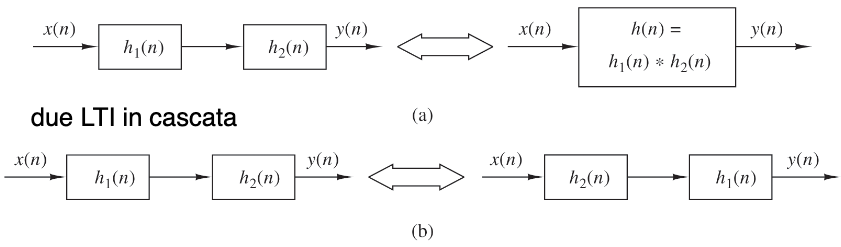
\includegraphics[scale=0.4]{Lezioni/Immagini/associativa}
\end{figure}

Per la proprietà distributiva, due LTI $h_1(n)$ e $h_2(n)$ connessi in parallelo possono essere sostituiti da un singolo sistema $h(n) = h_1(n) + h_2(n)$.

L'interazione del segnale nel sistema è il prodotto delle trasformate di Fourier, semplificando la convoluzione. $H$ è la risposta dell'impulso, che interagisce con $X$ per generare $Y$.  

Per il teorema della convoluzione, 
$$y(n) = x(n) * h(n) \leftrightarrow Y(f) = X(f)H(f) \quad \text{dove}\quad H(f) = \frac{1}{M} \sum_{n=0}^{M-1} h(n) e^{-j\frac{2\pi}{M}fn}$$
$$y(n) = x(n) * h(n) \leftrightarrow Y(e^{j\omega}) = X(e^{j\omega}) H(e^{j\omega})$$

La funzione continua $H(e^{j\omega})$ (trasformata discreta di $h(n)$) viene detta \textbf{risposta in frequenza} del sistema LTI, e può essere definita come:
$$H(e^{j\omega}) = \frac{Y(e^{j\omega})}{X(e^{j\omega})} = \Re(H(e^{j\omega})) + j(H(e^{j\omega})) = \abs{H(e^{j\omega})} e^{j\phi(H(e^{j\omega}))}$$

\subsection{Filtri}
Dato un generico sistema con una funzione $H(e^{j\omega})$, un \textbf{filtro} taglia alcune componenti in frequenza del segnale di ingresso lasciandone passare altre, secondo quanto specificato attraverso la risposta. 

Le frequenze nell'intervallo vengono moltiplicate per 1, le altre per 0. Ci sono diverse tipologie di filtri ideali: passa-basso, passa-alto, passa-banda o attenua-banda, che corrispondono alla funzione $sinc$ che è anticausale, pertanto non rappresentabile. 

$$\text{Filtro ideale passa-basso } \abs{H(e^{j\omega})} = \begin{cases}
1, & \abs{\omega} \leq \omega_t \\
0, & \omega_t < \abs{\omega} \leq \pi
\end{cases}$$
$$\text{Filtro ideale passa-alto } \abs{H(e^{j\omega})} = \begin{cases}
0, & \abs{\omega} \leq \omega_t \\
1, & \omega_t < \abs{\omega} \leq \pi
\end{cases}$$
$$\text{Filtro ideale passa-banda } \abs{H(e^{j\omega})} = \begin{cases}
0, & \abs{\omega} \leq \omega_1 \\
1, & \omega_1 < \abs{\omega} \leq \omega_2 \\
0, & \omega_2 < \abs{\omega} \leq \pi
\end{cases}$$
$$\text{Filtro ideale attenua-banda } \abs{H(e^{j\omega})} = \begin{cases}
0, & \abs{\omega} \leq \omega_1 \\
1, & \omega_1 < \abs{\omega} \leq \omega_2 \\
0, & \omega_2 < \abs{\omega} \leq \pi
\end{cases}$$

I sistemi LTI a tempo discreto devono soddisfare alcune condizioni specifiche, al fine di poter essere impiegati in alcune applicazioni. Una di queste condizioni è la stabilità, di cui la più usata nella pratica è detta \textbf{BIBO} (Bounded-Input Bounded-Output).

Un sistema rispetta la stabilità BIBO se, per ogni ingresso $h(n)$ con energia limitata, anche l'output ha ampiezza limitata (non va a infinito, è sommabile in modulo). $sinc$ tende a infinito, quindi non è stabile. 
$$h_s = \sum_{-\infty}^{+\infty} \abs{h(n)} < \infty$$
Un sistema LTI è fisicamente realizzabile se possiede una risposta all'impulso $h(n)$ reale e causale, dove la causalità implica $h(n) = 0\ \forall\ n < 0$.

La funzione di trasferimento $H$ nel dominio delle frequenze di un filtro ideale passa-basso possiede le seguenti caratteristiche:
\begin{itemize}
	\item $\abs{H}$ costante nella banda passante e nullo nella banda proibita;
	\item La banda passante e la banda proibita sono confinanti, separate dalla \textit{frequenza di taglio}.
\end{itemize}

Un filtro reale, in confronto a uno ideale, non ha zone ben precise di banda passante e probita: la transizione non è immediata (esiste una zona di transizione) e le frequenze non hanno peso uguale bensì fluttuazioni con ampiezza variabile. 

Si rilevano oscillazioni non trascurabili ampie $\delta_1$. L'attenuazione si calcola come $20\log_{10} \delta_2\ dB$, con $\delta_2$ ampiezza della massima oscillazione in banda proibita. 

La banda passante e la banda proibita sono separate appunto dalla \textbf{banda di transizione}, che inizia dalla frequenza di taglio $v_c$ e termina alla frequenza di stop $v_s$ (dimensione $v_s - v_c$). Questi parametri vengono dati come specifiche dei filtri. 

\begin{wrapfigure}{L}{0.55\textwidth}
	\vspace{-15pt}
	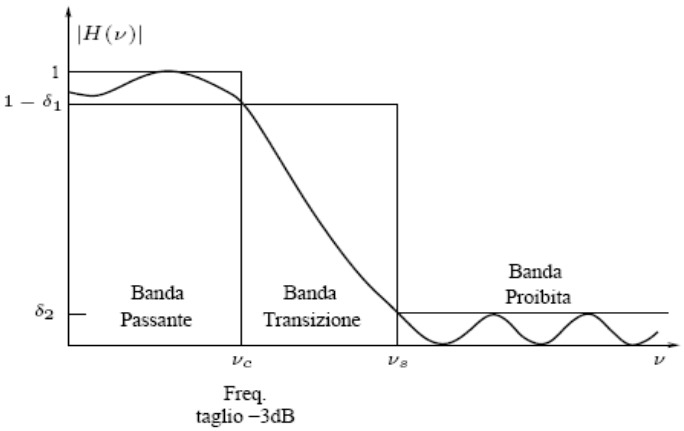
\includegraphics[width=0.55\textwidth]{Lezioni/Immagini/taglio}
	\vspace{-50pt}
\end{wrapfigure}

La frequenza di taglio è la frequenza per la quale la potenza è il 50\% rispetto al massimo, quindi c'è un'attenuazione della metà. Serve per identificare la fine della banda passante. Se $\abs{H(v)}^2 \approx 1$, $v_c$ è la frequenza per cui:
$$\abs{H(v_c)}^2 = \frac{1}{2}$$
$v_c$ è anche detta frequenza di taglio a 3 dB poichè $10\log_{10}(\nicefrac{1}{2}) \approx -3\ dB$.
\bigskip
\bigskip